\documentclass{beamer}
\usetheme{}
\usecolortheme{dolphin}           
\useinnertheme{circles}
\setbeamertemplate{itemize items}[default]
\setbeamertemplate{enumerate items}[default]
\usepackage[T1]{fontenc}
\usepackage[utf8]{inputenc}
\usepackage{lmodern}
\usepackage{amsmath}
\usepackage{booktabs} 
\usepackage{graphicx}        
\usepackage{array}
\usepackage{color}
\makeatletter
\def\zapcolorreset{\let\reset@color\relax\ignorespaces}
\def\colorrows#1{\noalign{\aftergroup\zapcolorreset#1}\ignorespaces}
\makeatother
\graphicspath{{/home/swl/Dropbox/ucd/advanced_macro/figures/}} 
\setbeamertemplate{navigation symbols}{}
\setbeamertemplate{footline}[frame number]

%--------------------------------------
\title{Estimating DSGE models}
\author{School of Economics, University College Dublin}
\date{Spring 2018}
\begin{document}

%--------------------------------------
\begin{frame}
 \titlepage
\end{frame}
%--------------------------------------

%--------------------------------------
\begin{frame}
 Example frequentism
\end{frame}
%--------------------------------------


%--------------------------------------
\begin{frame}
 DSGE models are complex; early models were calibrated
 \begin{itemize}
     \item Picking parameter values that match steady-state values
     \begin{itemize}
       \item Labour share of income; capital-output ratio; etc. 
     \end{itemize}
     \item Combine with historical averages
     \item Parameter estimates from microeconomic studies 
     \begin{itemize}
       \item Relative risk aversion; labour supply elasticities; depreciation rates
     \end{itemize}
   \end{itemize}  
   \medskip
   Alternatively there was \textbf{indirect inference}: choosing parameters to match certain data moments
\end{frame}
%--------------------------------------

%--------------------------------------
\begin{frame}
  Number of issues to cover concerning DSGE model estimation\medskip  
\begin{enumerate}
  \item Divide model into observable and unobservable variables
  \item Role played by shocks in the model
  \item State-space models estimated with Kalman filter
  \item Bayesian methods
\end{enumerate}
\end{frame}
%--------------------------------------

%--------------------------------------
\begin{frame}
  \textbf{Solved model}  
\begin{align}  
  KZ_t = AZ_{t-1} + BE_tZ_{t+1} + HX_t 
\end{align}
$Z_t$ is a set of $n$ endogenous variables\\
$X_t$ is a set of $k$ exogenous variables; evolves according to 
\begin{align}
  X_t=DX_{t-1}+\epsilon_t
\end{align}
\medskip
Solution of model given by
\begin{align}  
  Z_t=CZ_{t-1}+PX_t 
\end{align}
$C$ depends on the coefficients in $A,B$\\
$P$ depends on the coefficients in $A,B,H,D$.
\end{frame}
%--------------------------------------

%--------------------------------------
\begin{frame}
 \begin{align*}  
 KZ_t &= AZ_{t-1} + BE_tZ_{t+1} + HX_t\\
 X_t&=DX_{t-1}+\epsilon_t\\  
 Z_t&=CZ_{t-1}+PX_t 
\end{align*}
 To establish model's properties could simulate it
 \begin{itemize}
   \item But we are interested in the estimates of the coefficients in $A, B, D, H$
   \item Estimation depends on type of data we have
 \end{itemize} 
\end{frame}
%--------------------------------------


%--------------------------------------
\begin{frame}
  \textbf{Observable variables}\\
  Suppose all variables in $X_t,Z_t$ are observable: model makes a clear prediction that given any set of structural parameter $A,B,H,D$, the data will be given by
\begin{align*}  
  Z_t=CZ_{t-1}+PX_t 
\end{align*}
\end{frame}
%--------------------------------------

%--------------------------------------
\begin{frame}
  Likely that there is no set of $A,B,D,H$ matrices that will allow the model to fit the data perfectly
  \begin{itemize}
    \item Cross-equation restrictions in DSGE models
    \item Particular patterns must be observed by $C,P$
    \item Cannot use MLE as a results
  \end{itemize}
  Can add error terms $u_t$ to estimate $A, B, D, H$ 
\begin{align}
  Z_t=CZ_{t-1} + PX_t + u_t
\end{align}
$u_t$ does not have any microeconomic foundation, but it will provide a sense of how well the model fits the data.
\end{frame}
%--------------------------------------

%--------------------------------------
\begin{frame}
  Can use MLE when we have model with observable variables  
\begin{align}  
  Z_t&=CZ_{t-1} + PX_t + u_t\\
  X_t &= DX_{t-1} + \epsilon_t\\
  u_t&\sim N(0,\sum\nolimits_u)\\
  \epsilon_t&\sim N(0,\sum\nolimits_\epsilon)
\end{align}
\medskip
 Suppose endogenous variables are observed by $Z_1,Z_2,......,Z_T$; exogenous variables by $X_1,X_2,......,X_T$
 \begin{itemize}
    \item Can combine log-likelihood functions for the $Z$ and $X$ data as the likelihood of the full model multiplies the likelihood of the $X$ data and the likelihood of the $Z$ data 
  \end{itemize} 
\end{frame}
%--------------------------------------

%--------------------------------------
\begin{frame}
 Maximum likelihood estimates of $A,B,H,D,\sum\nolimits_{\epsilon}, \sum\nolimits_u$ are those that maximise the following log-likelihood
\begin{align}
  -T\;log2\pi - T (log |\sum\nolimits_\epsilon^{-1}| + log |\sum\nolimits_u^{-1}|)\\
  - \frac{1}{2}\sum\nolimits_{k=1}^T(X_i-DX_{i-1})'\sum\nolimits_\epsilon^{-1}(X_i-DX_{i-1})\\
  -\frac{1}{2}\sum\nolimits_{k=1}^T(Z_i-CZ_{i-1}-PX_i)'\sum\nolimits_u^{-1}(Z_i-CZ_{i-1}-PX_i)  
\end{align}
Subject to the restrictions that map $A$ and $B$ into $C$ and map $A,B,H,D$ into $P$.  
\end{frame}
%--------------------------------------

%--------------------------------------
\begin{frame}
  One issue: Most DSGE models do not exclusively rely on observable variables
  \begin{itemize}
    \item Mix of observable and unobservable variables. 
  \end{itemize}
  \medskip
  Consider standard RBC model
\begin{align*}
  y_t &= \left(1-\frac{\alpha \gamma}{\beta^{-1}+\gamma -1}\right)c_t +
  \left(\frac{\alpha \gamma}{\beta^{-1}+\gamma-1}\right)i_t\\
  y_t &= a_t +\alpha k_{t-1} + (1-\alpha)n_t\\
  k_t &= \gamma i_t + (1-\gamma)k_{t-1}\\
  n_t &= y_t-\eta c_t\\
  c_t &= E_t c_{t+1} - \frac{1}{\eta}E_t r_{t+1}\\
  r_t &= (1-\beta(1-\gamma))(y_t-k_{t-1})\\
  a_t &= \rho a_{t-1} + \epsilon_t
\end{align*}
\end{frame}
%--------------------------------------

%--------------------------------------
\begin{frame}
  Model features 7 equations with 6 endogenous variables and one exogenous variable
\begin{itemize}
  \item Endogenous: $y_t,c_t,i_t,k_t,n_t,r_t$
  \item Exogenous: $a_t$
\end{itemize}
\medskip
The model also mixes 4 observable variables and three unobservable variables
\begin{itemize}
  \item Observable: $y_t,c_t,i_t,n_t$
  \item Unobservable: $a_t, k_t, r_t$
\end{itemize}
Issue in RBC model: All observed series depend on unobservable technology series\\
In order to deal with the unobservable variables, special techniques are required. 
\end{frame}
%--------------------------------------

%--------------------------------------
\begin{frame}
  RBC model features stochastic shocks but also \textbf{stochastic singularity}
  \begin{itemize}
    \item shocks in all the equations are just multiples of each other. 
    \item The model will therefore predict that certain ratios of the observed variables will be constant, while in reality these predictions do not hold    
  \end{itemize}
  Result: model won't fit the data
\end{frame}
%--------------------------------------

%--------------------------------------
\begin{frame}
 For a model to have well-defined econometric estimates it is therefore necessary that for every observable variable there is at least one unobservable shock. 
This can take in shape in two different forms
\begin{enumerate}
  \item measurement error
  \item involve a shock in each equation with a clear structural interpretation
\end{enumerate}
\end{frame}
%--------------------------------------

%--------------------------------------
\begin{frame}
  A DSGE model that is a mix of observable and unobservable variables is an example of state-space model. 
This type model can be described using two equations
\begin{enumerate}
  \item the state (transition) equation $S_t$
  \item the measurement equation $Z_t$
\end{enumerate}
\begin{align*}
    S_t &= FS_{t-1} + u_t\\
    Z_t &= HS_t+v_t
\end{align*}
The error terms $u_t,v_t$ can include normally distributed errors or zeroes if the equation described is an identity.
\end{frame}
%--------------------------------------

%--------------------------------------
\begin{frame}
 RBC model (without labour input)  
\begin{align}
  k_t &= a_{kk}k_{t-1} + a_{kz}z_t\\
  c_t &= a_{ck}k_{t-1} + a_{cz}z_t\\
  z_t &= \rho z_{t-1} + \epsilon_t
\end{align}
For the sake of the illustration let's assume that consumption and capital are only observed with error, this makes that the two observable variables are
\begin{align}
  k_t^* &= a_{kk}k_{t-1} + a_{kz}z_t + u_t^k\\
  c_t^* &= a_{ck}k_{t-1} + a_{cz}z_t + u_t^c\\  
\end{align}
\end{frame}
%--------------------------------------


%--------------------------------------
\begin{frame}
  This can be written in state-space form using the transition and measurement equation
\begin{align}
  \begin{pmatrix} k_{t-1} \\ z_t  \end{pmatrix} &= 
  \begin{pmatrix} a_{kk} & a_{kz} \\ 0 & \rho \end{pmatrix}
  \begin{pmatrix} k_{t-2} \\ z_{t-1} \end{pmatrix} +
  \begin{pmatrix} 0 \\ \epsilon_t \end{pmatrix}\\
  \begin{pmatrix} k^*_{t-1} \\ c^*_t \end{pmatrix} &=
  \begin{pmatrix} 1 & 0 \\ a_{ck} & a_{cz}  \end{pmatrix}
  \begin{pmatrix} k_{t-1} \\ z_t \end{pmatrix} +
  \begin{pmatrix} u^k_{t-1} \\ u^c_t \end{pmatrix}
\end{align}
Some adjustments had to be made to get the model in state-space form and the timing conventions associated with this representation are not quite the same as in the original model.

\end{frame}
%--------------------------------------

%--------------------------------------
\begin{frame}
  Here we get that
\begin{align}
  S_t &= \begin{pmatrix} k_{t-1} \\ z_t  \end{pmatrix}\\
  Z_t &= \begin{pmatrix} k^*_{t-1} \\ c^*_t \end{pmatrix}
\end{align}
This can be used for all DSGE models which can be estimated using the Kalman filter. 
\end{frame}
%--------------------------------------

%--------------------------------------
\begin{frame}
  Using the Kalman filter one can actually estimate a DSGE model that mixes observable and unobservable variables using MLE. 
Once you have specified the model you can feed it into a computer package which will 
\begin{enumerate}
  \item Sort the model into space-state methods
  \item Find possible parameter values 
  \item Use Kalman filter to smooth parameters
  \item Produce period-by-period likelihoods for possible parameter values
  \item Pick best parameters and calculate standard errors (using MLE)  
\end{enumerate}

\end{frame}
%--------------------------------------

%--------------------------------------
\begin{frame}
  Using MLE is not without dangers however. 
Some of the issues with maximising the likelihood of a DSGE include
\begin{itemize}
  \item Large number of parameters
  \item Sparsity of data (often quarterly)
  \item Flexible nature of DSGE, generating similar behaviour with different parameter values
  \item Standard errors difficult to compute
\end{itemize}
\end{frame}
%--------------------------------------

%--------------------------------------
\begin{frame}
\scalebox{.7}{
  \begin{quote}
    maximizing a complicated, highly dimensional function like the likelihood of
a DSGE model is actually much harder than it is to integrate it, which is what
we do in a Bayesian exercise. First, the likelihood of DSGE models is, as I
have just mentioned, a highly dimensional object, with a dozen or so
parameters in the simplest cases to close to a hundred in some of the richest
models in the literature. Any search in a high dimensional function is fraught
with peril. More pointedly, likelihoods of DSGE models are full of local
maxima and minima and of nearly flat surfaces. This is due both to the
sparsity of the data (quarterly data do not give us the luxury of many
observations that micro panels provide) and to the flexibility of DSGE models
in generating similar behavior with relatively different combination of
parameter values .... Moreover, the standard errors of the estimates are
notoriously difficult to compute and their asymptotic distribution a poor
approximation to the small sample one
  \end{quote}}\\
  \medskip
  From \textit{"The econometrics of DSGE models"}, Fernandez-Villaverde
\end{frame}
%--------------------------------------

%--------------------------------------
\begin{frame}
Due to this difficulties, most current research prefers to use Bayesian methods. 
The Bayesian approach specifies a prior likelihood which will be combined with the likelihood function to produce an estimate of the posterior. 
Once the posterior is calculated it is relatively straightforward to produce means, confidence intervals, etc. 
The main advantage of the Bayesian approach over MLE is that it uses a full likelihood function rather than a single point estimate. 
One important question concerning the use of Bayesian method is of course how the prior is determined. 
In practice the prior is defined using a distribution in the form that fits common sense and corresponds to previous studies. 
\end{frame}
%--------------------------------------

%--------------------------------------
\begin{frame}
  First: data
  \begin{align}
    y^T \equiv \{y_t \}^T_{t=1} \in \mathbb{R}^{N\times T}
  \end{align}
  Second: model
  \begin{align}
    i \in M
  \end{align}
  Model composed by
  \begin{enumerate}
    \item Parameter set
    \begin{align}
      \Theta_i \in \mathbb{R}^{k_i}
    \end{align}
    \item Likelihood function
    \begin{align}
      p(y^T | \theta,i): \mathbb{R}^{N\times T} \times \Theta_i \rightarrow \mathbb{R}^+
    \end{align}
    \item Prior distribution
    \begin{align}
      \pi(\theta|i): \Theta_i \rightarrow \mathbb{R}^+
    \end{align}
  \end{enumerate}
\end{frame}
%--------------------------------------

%--------------------------------------
\begin{frame}
 Posterior distribution of parameters given by
 \begin{align}
   \pi(\theta|y^T, i) = \frac{p(y^T|\theta,i)\pi(\theta|i)}{\int p(y^T|\theta,i)\pi(\theta|i)d\theta}.
 \end{align}
  In short: Prior beliefs $\pi(\theta|y^T, i)$ are combined with sample information $f(y^T|\theta,i)$ to arrive at new beliefs $\pi(\theta|y^T,i)$
\end{frame}
%--------------------------------------

%--------------------------------------
\begin{frame}
  \begin{figure}
    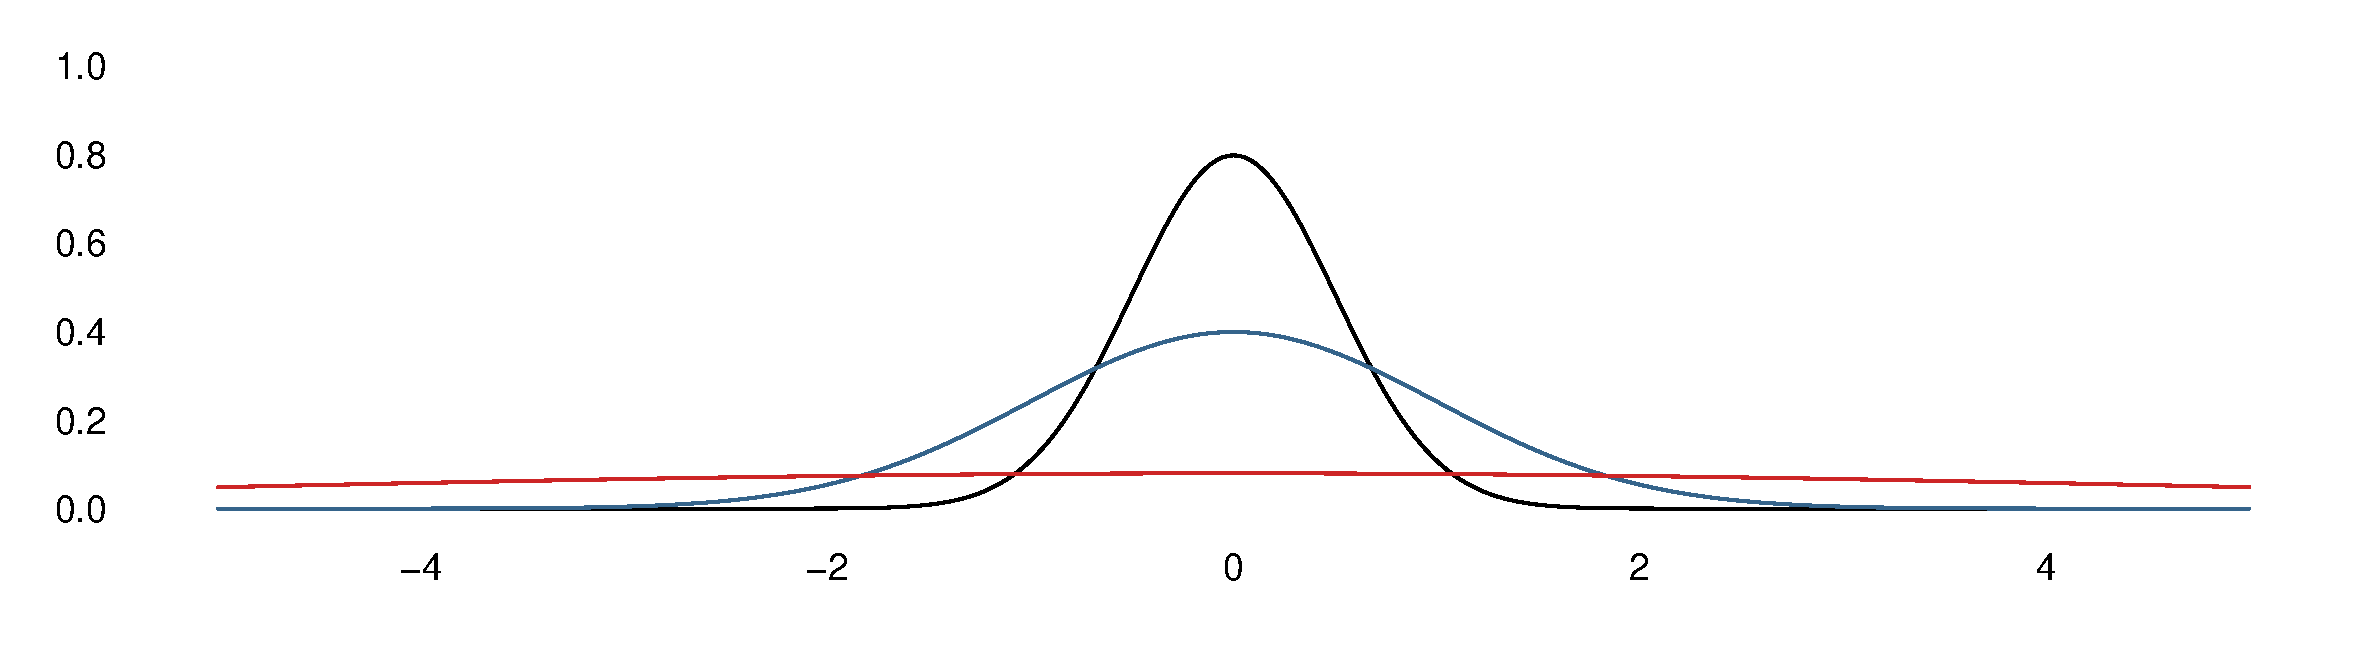
\includegraphics[scale=.3]{prior_normal.eps}
  \end{figure}
\end{frame}
%--------------------------------------

%--------------------------------------
\begin{frame}
\begin{figure}
    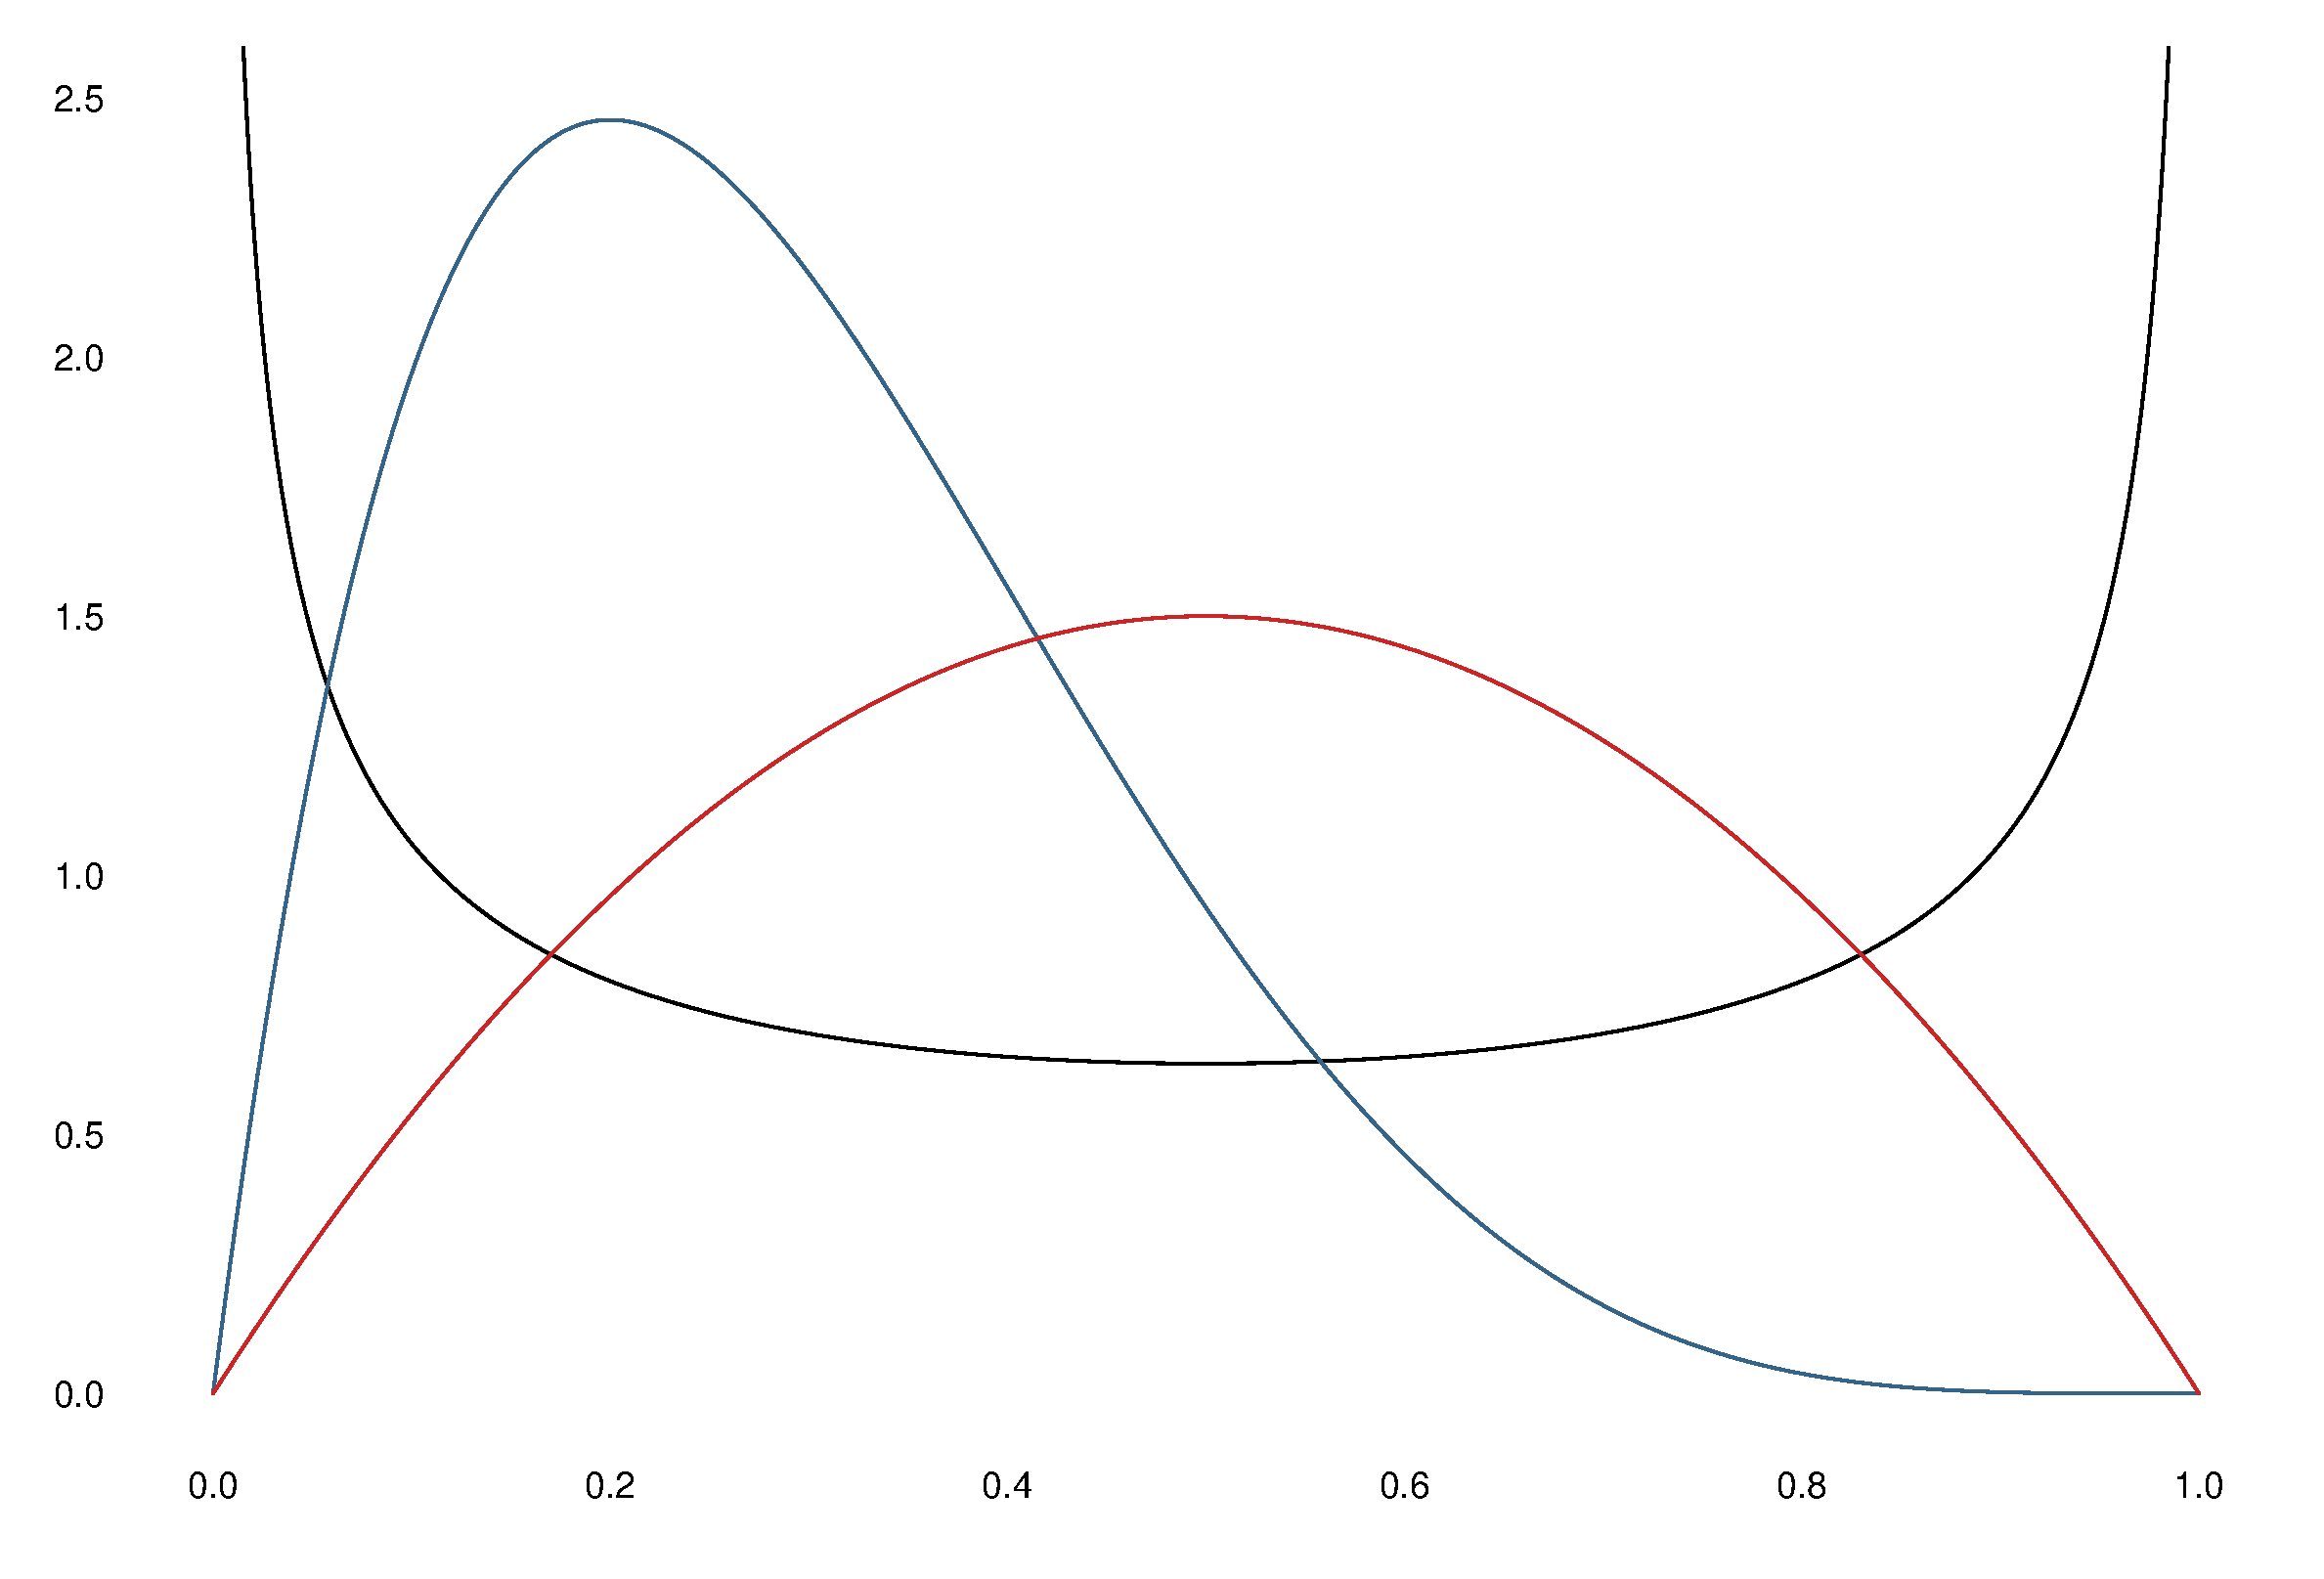
\includegraphics[scale=.3]{prior_beta.eps}
  \end{figure}
\end{frame}
%--------------------------------------

%--------------------------------------
\begin{frame}
\begin{figure}
    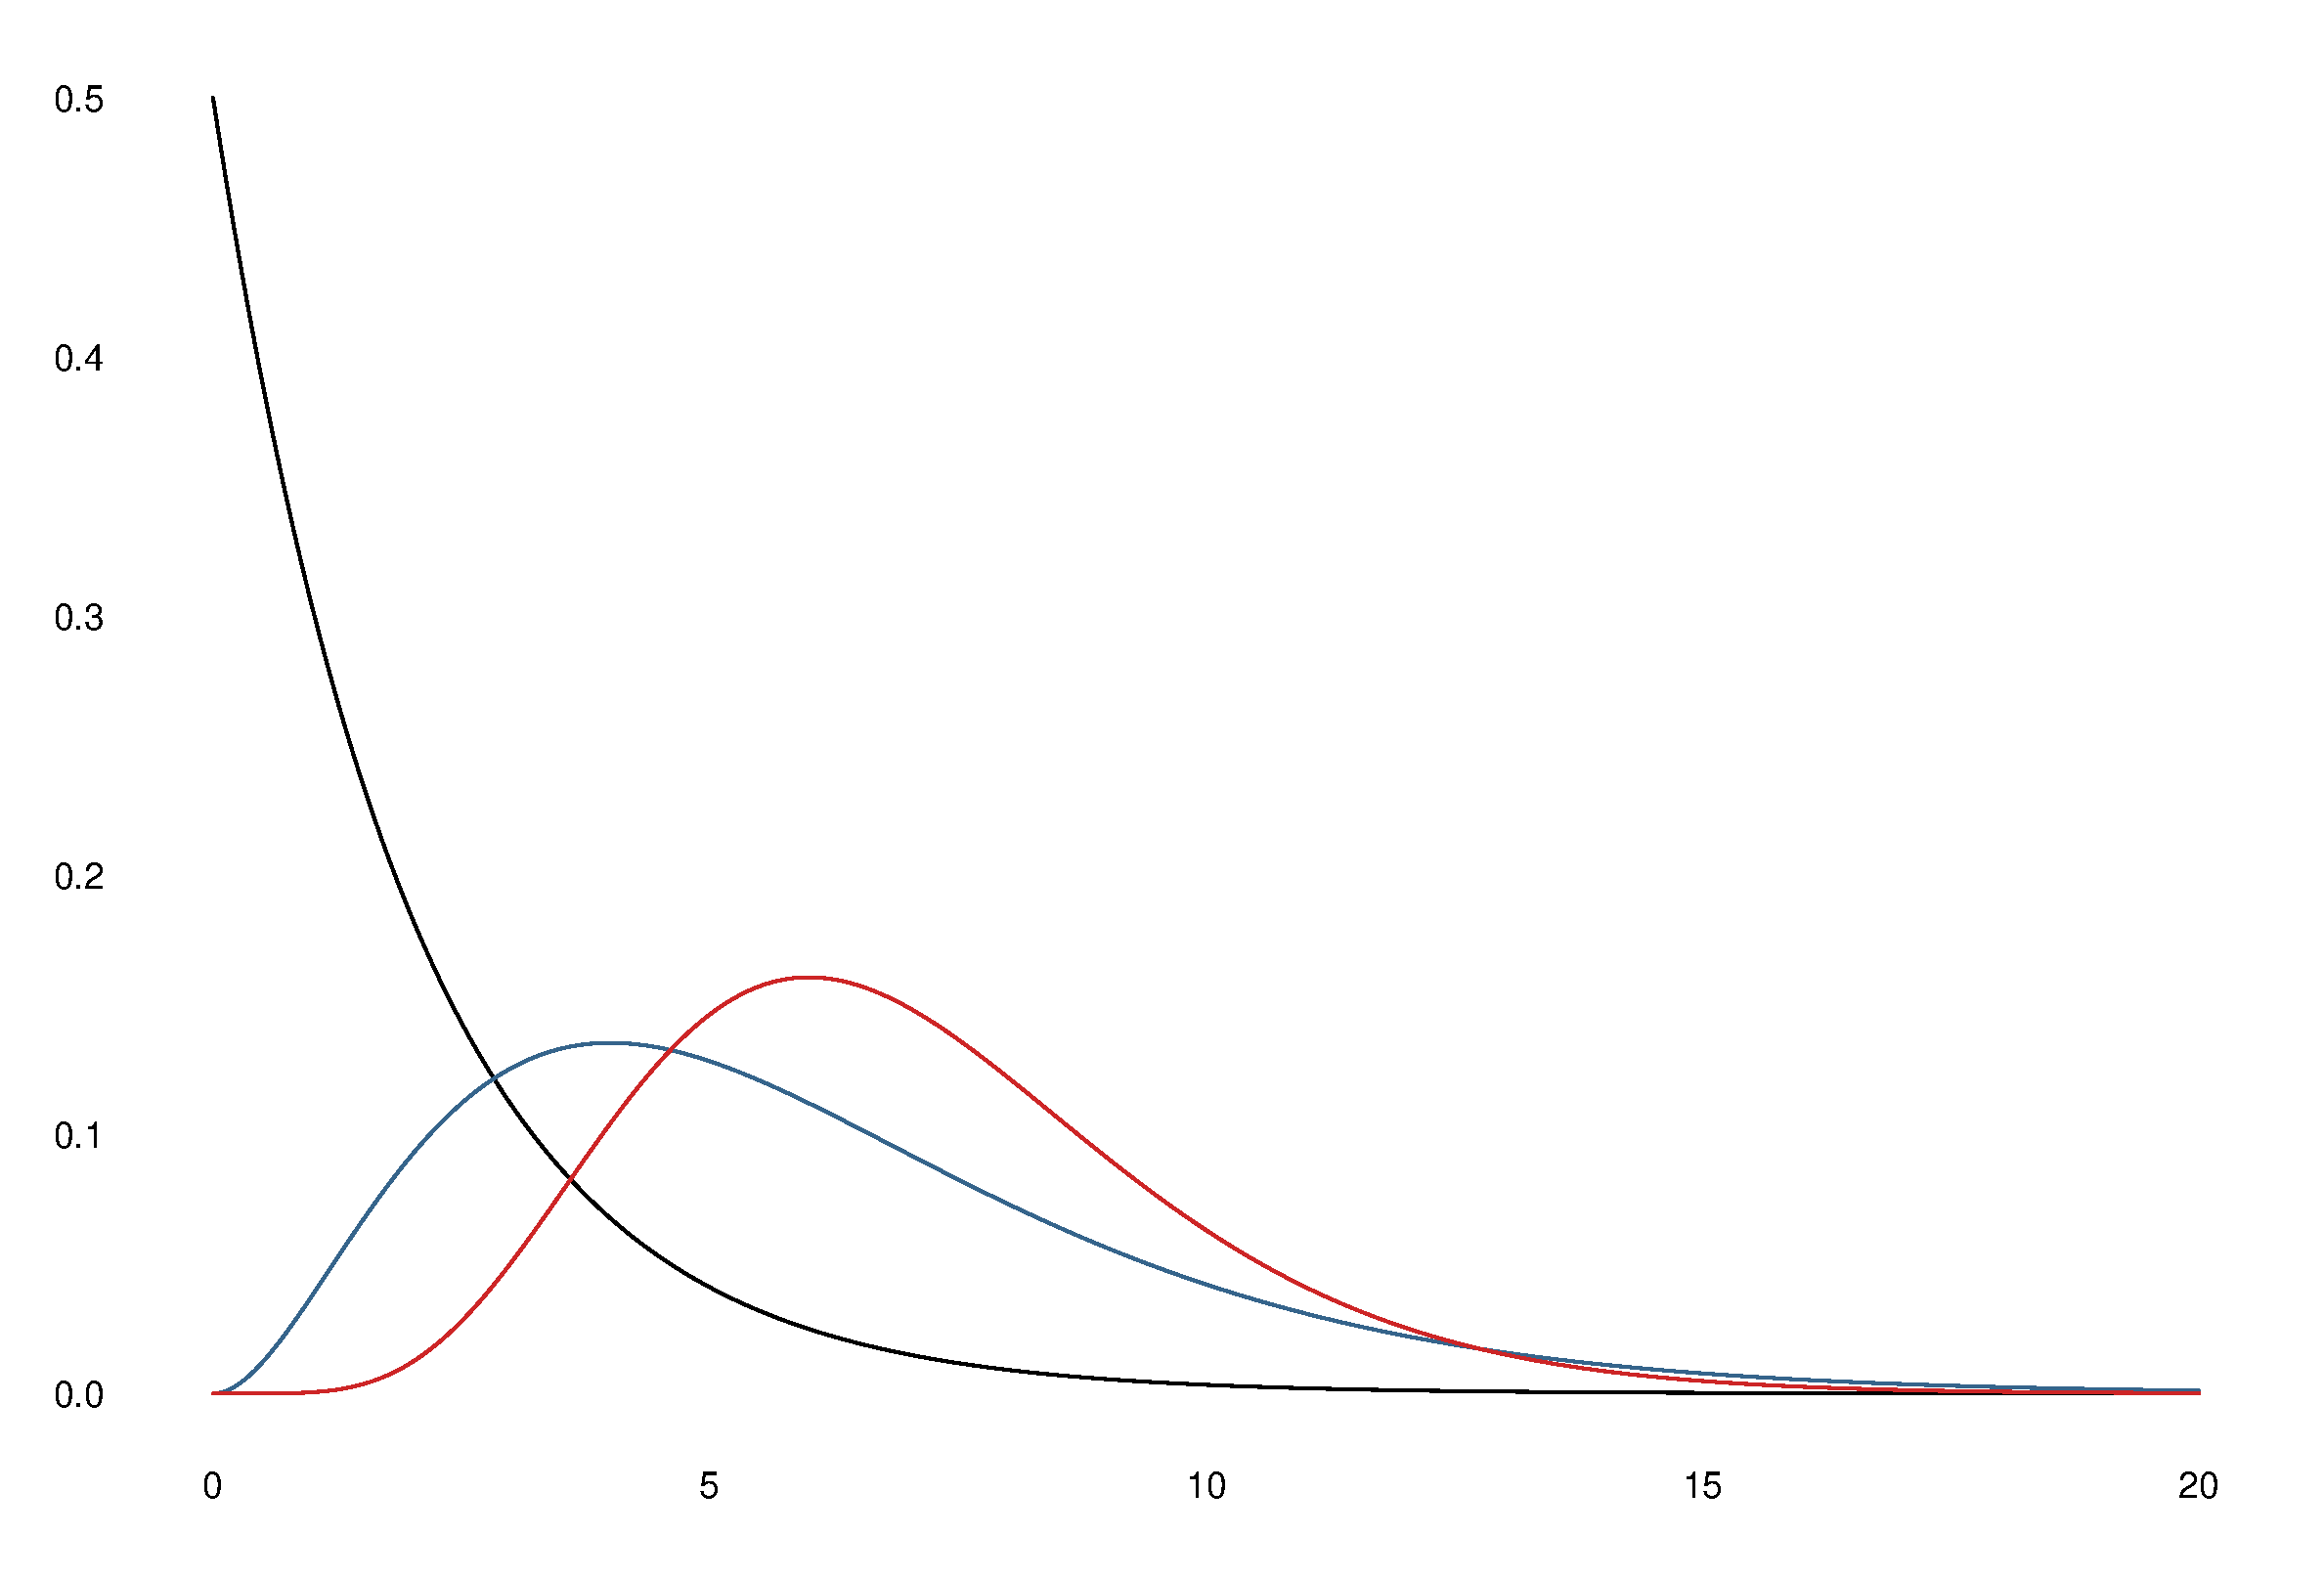
\includegraphics[scale=.3]{prior_gamma.eps}
  \end{figure}
\end{frame}
%--------------------------------------


%--------------------------------------
\begin{frame}
  \begin{enumerate}
    \item User-relevant answers
    \item Can use pre-sample information
    \item Direct computation of objects of interests
    \item Ease to deal with misspecified models
  \end{enumerate}
  \begin{enumerate}
    \item Other methods provide more transparent link with FOCs and equilibrium equations
    \item Still can be computationally intensive
  \end{enumerate}
\end{frame}
%--------------------------------------

%--------------------------------------
\begin{frame}
 Need right set of tools
 \begin{enumerate}
   \item Solution methods
   \item Method to evaluate likelihood of model
   \item Method to explore likelihood of model
 \end{enumerate}
\end{frame}
%--------------------------------------

%--------------------------------------
\begin{frame} 
  No analytical solutions
  \begin{itemize}
    \item Need numerical approximations
  \end{itemize}
  \medskip
  \begin{enumerate}
    \item Substitute difficult original problem with simpler one
    \item Use solution to approximate solution of original problem
  \end{enumerate}
  In DSGE: Taylor expansion of function describing variable dynamics around deterministic steady-state
\end{frame}
%--------------------------------------


%--------------------------------------
\begin{frame}
  \textbf{State-space model}
  \begin{enumerate}
    \item Transition equation
    \begin{align*}
      S_t=f(S_{t-1}, W_t; \theta)
    \end{align*}
    \item Measurement equation
    \begin{align*}
      Y_t=g(S_t, V_t;\theta)
    \end{align*}
  \end{enumerate}
  \medskip
  Measurement equation subject to one restriction
  \begin{enumerate}
    \item Can only select number of series less or equal than number of shocks ($W_t,V_t$)
  \end{enumerate}
  Otherwise it will be stochastically singular: likelihood $-\infty$ with probability 1
\end{frame}
%--------------------------------------

%--------------------------------------
\begin{frame}
  Compute
  \begin{align}
    S_t=f(S_{t-1}, W_t; \theta) &\rightarrow p(S_t|S_{t-1};\theta)\\
    Y_t=g(S_t, V_t;\theta) &\rightarrow p(Y_t|S_t;\theta)\\
    Y_t=g(f(S_{t-1},W_t;\theta),V_t;\theta) &\rightarrow p(Y_t|S_{t-1};\theta)
  \end{align}
  
\end{frame}
%--------------------------------------

%--------------------------------------
\begin{frame}
  \begin{align}
   p(Y^T|\theta) &= p(y_1|\theta) \prod^T_{t=2}p(y_t|y_{t-1};\theta)\\
   &= \int(p(y_1|s_1;\theta)dS_1\prod^T_{t=2} \int p(y_t|S_t;\theta) p(S_t|Y_{t-1};\theta)dS_t
  \end{align}
  Can therefore evaluate likelihood of model when we have knowledge of
  \begin{align}
    \{p(S_t|y_{t-1};\theta \} ^T_{t-1}\\
    p(S_1;\theta)
  \end{align} 
\end{frame}
%--------------------------------------

%--------------------------------------
\begin{frame}
  \textbf{Chapman-Kolmogorov equation}
  \begin{align}
    p(S_{t+1}|y_t;\theta)=\int p(S_{t+1}|S_t;\theta)p(S_t|y_t;\theta)dS_t
  \end{align}
  Provides forecasting rule for the evolution of states
  \begin{quote}
    The distribution of states tomorrow, given the states until today, is equal to the distribution of states today times the transition probabilities integrated over all possible states
  \end{quote}
\end{frame}
%--------------------------------------

%--------------------------------------
\begin{frame}
  \textbf{Bayes theorem} once again
  \begin{align}
    p(S_t|y_t;\theta)&=\frac{p(y_t|S_t;\theta)p(S_t|y_{t-1};\theta)}{p(y_t|y_{t-1};\theta)}\\
    p(y_t|y_{t-1};\theta) &= \int p(y_t|S_t;\theta)p(S_t|y_{t-1};\theta)dS_t
  \end{align}
\end{frame}
%--------------------------------------

%--------------------------------------
\begin{frame}
  Using Chapman-Kolmogorov equation and Bayes Theorem can generate complete sequence for
  \begin{align}
    \{p(S_t|y_{t-1};\theta\}^T_{t=1}
  \end{align}
  \medskip
  Mathematically straightforward; practically difficult: Can fix computational problem
  \begin{enumerate}
    \item Kalman filter
    \item Particle filter
    \begin{itemize}
      \item Use when state-space representation is not linear or shocks are not normal
    \end{itemize}
  \end{enumerate}
\end{frame}
%--------------------------------------

%--------------------------------------
\begin{frame}
  \textbf{Exploring the likelihood function}
  \begin{enumerate}
    \item Maximisation
    \item Description
  \end{enumerate}
  Can also just use posterior distribution
  \begin{align}
    \pi(\theta|y_t) = \frac{p(y_t|\theta)\pi(\theta)}{\int p(y_t|\theta)\pi(\theta)d\theta}
  \end{align}
  Use Markov Chain Monte Carlo methods
  \begin{itemize}
    \item Metropolis-Hastings algorithm
    \item Gibbs sample (special case of (1))
  \end{itemize}
\end{frame}
%--------------------------------------

%--------------------------------------
\begin{frame}
  \textbf{Metropolis-Hastings algorithm}
  \begin{figure}
    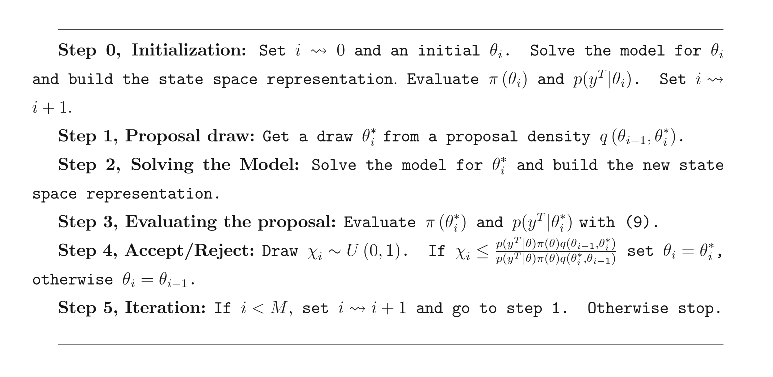
\includegraphics[scale=.8]{metropolis.eps}
  \end{figure}
\end{frame}
%--------------------------------------


%--------------------------------------
\end{document}
